
% APPENDIX 
\setcounter{table}{0}
\setcounter{figure}{0}
\setcounter{section}{0}
\pagenumbering{gobble}

\begin{center}
	\LARGE Does Seguro Popular Reduce Formal Jobs?  \\[0.5em]
	\Large{Appendix $-$ For Online Publication} \\[1em]
	\large \author{Enrique Seira  \and Isaac Meza  \and Eduardo González-Pier \and Eduardo Alcaraz}
\end{center}

\appendix
\pagenumbering{arabic}
\renewcommand\thefigure{OA-\arabic{figure}}
\renewcommand\thetable{OA-\arabic{table}}
\renewcommand*{\thepage}{OA - \arabic{page}}
\renewcommand\thesection{Appendix \Alph{section}.}
\renewcommand\thesubsection{\Alph{section}.\arabic{subsection}}

%\renewcommand{\cftparskip}{0em} % NOT NEEDED
\renewcommand\cftsecdotsep{\cftdotsep}
\renewcommand\cftsubsecdotsep{\cftnodots}
\renewcommand{\cftsecnumwidth}{6em}
 \renewcommand{\cftpnumalign}{r}
%\renewcommand{\cftsecleader}{\normalfont\cftdotfill{\cftsecdotsep}}


\renewcommand{\cftsecleader}{\cftdotfill{\cftsecdotsep}\hspace{1.8em}}
%\renewcommand{\cftsecpagefont}{20em}
%\renewcommand{\cftfignumwidth}{6em}
%\renewcommand{\cfttabnumwidth}{3.3em}

%\tableofcontents
\etocdepthtag.toc{mtappendix}
\etocsettagdepth{mtchapter}{none}
\etocsettagdepth{mtappendix}{subsection}

\setstretch{0.9}
%\renewcommand\contentsname{} % the empty name

\begingroup
\let\clearpage\relax
%\vspace{-1.5em} % the removed space. Set as appropriate
\tableofcontents
\endgroup


\newpage

\vspace{.2in}

\section{Additional Results}


\begin{figure}[H]
    \caption{Health expenditure as proportion of current income}
    \label{health_expenditure_share}
\begin{center}
\begin{subfigure}{0.60\textwidth}
        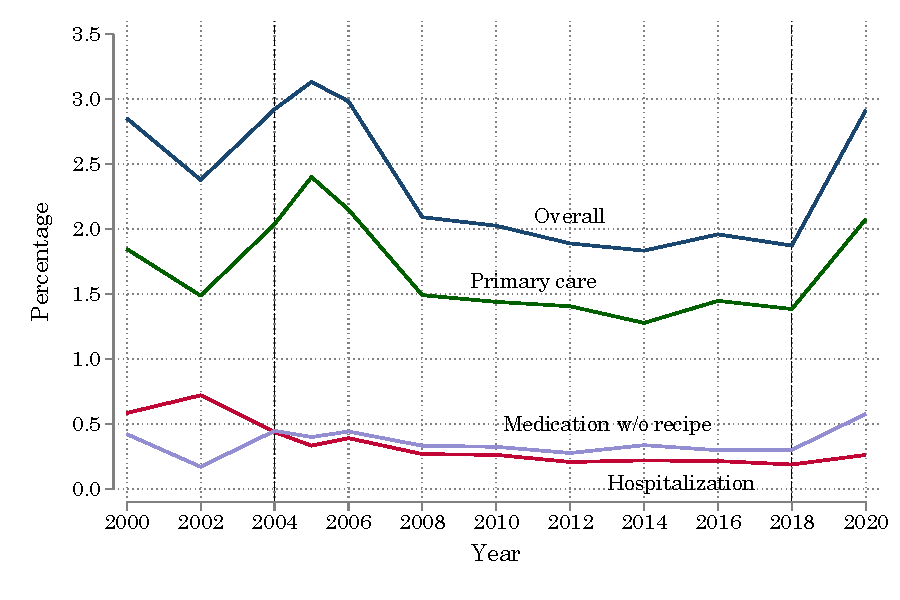
\includegraphics[width=\textwidth]{Figuras/oop_evolution_percentages.pdf}
    \end{subfigure}
 \end{center}
 \scriptsize 
    Vertical dashed lines denote beginning and ending of 
 SP program. This figure uses Mexico´s income and expenditure survey ENIGH - conducted by INEGI - from 2000 to 2020 to plot the mean health expenditure as proportion of a household's current income. To construct each variable we take the quarterly reported expenditure on each of the expenditure categories and make them annual quantities multiplying them by 4, as suggested by INEGI. We then standardize expenditure to 2018 Mexican pesos to make quantities comparable over time. Lastly, we divide each category's expenditure by the annualized current income to compute health expenditures as proportions of current income. For computing the mean we use frequency weights provided by INEGI in each survey. ENIGH data is collected every two years; in 2005 an additional survey was run in response to the demand for data by policymakers and researchers.
    %\scriptsize \textit{Scripts: }  \texttt{12_pocket_expenditure.do + aux_oop_graph.do}
\end{figure}

\vspace{.2in}



\subsection{TWFE diagnostics}
\begin{figure}[H]
     \caption{TWFE weights}
    \label{twfe_weights}
\begin{center}
       \begin{subfigure}{0.45\textwidth}
        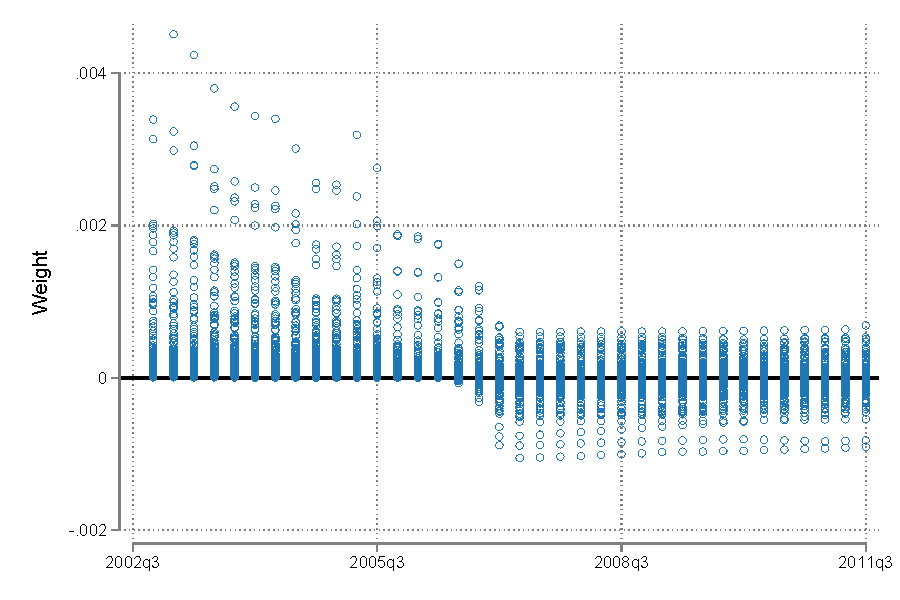
\includegraphics[width=\textwidth]{Figuras/twfe_w_p_t.pdf}
    \end{subfigure}
  \end{center}
    \scriptsize 
We compute the weights attached to the two-way fixed effects regressions studied in \cite{deChaisemartin_twfe_weight}, and using their STATA command - \textit{twowayfeweights}. Under the common trends assumption, beta estimates a weighted sum of 36741 ATTs. 26018 ATTs receive a positive weight, and 10723 receive a negative weight.
The sum of the positive weights is equal to 1.37.
The sum of the negative weights is equal to -0.37.
Observe that for the later quarters we find negative weights, so that the DiD estimates become biased for estimates 3-5 years after implementation. Exactly when \cite{Campos} find their larger effects.
%\textit{Scripts: }  \texttt{weights_twfe_diagnostic.do}
\end{figure}


\subsection{Replication \cite{Campos}}

\begin{figure}[H]
     \caption{Event studies - \cite{Campos} replication}
    \label{es_bc}
\begin{center}
       \begin{subfigure}{0.325\textwidth}
    \caption{Employers}
        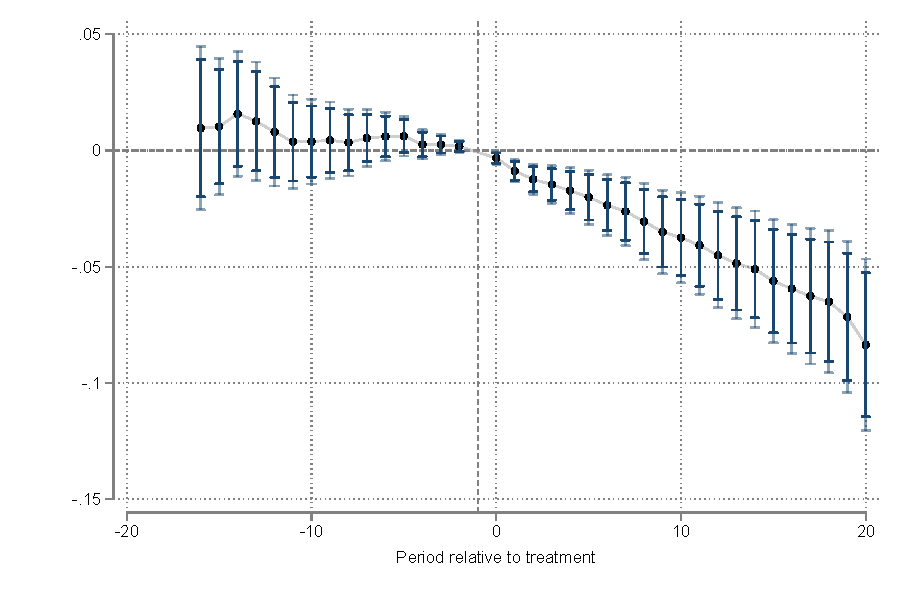
\includegraphics[width=\textwidth]{Figuras/did_event_bc_p_t.pdf}
    \end{subfigure}
    \begin{subfigure}{0.325\textwidth}
        \caption{Self-employed}
        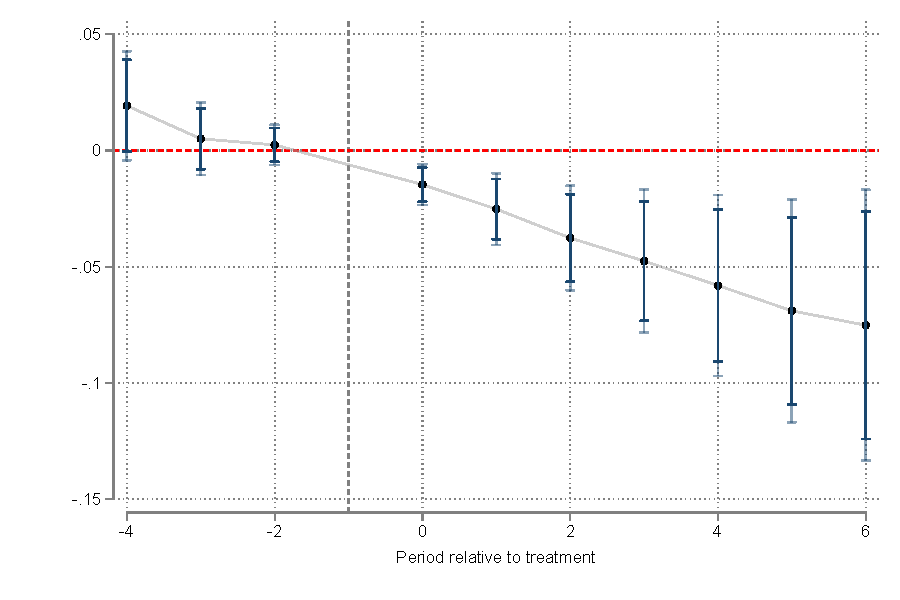
\includegraphics[width=\textwidth]{Figuras/did_event_bc_p_1.pdf}
    \end{subfigure}
        \begin{subfigure}{0.325\textwidth}
    \caption{Employees}
        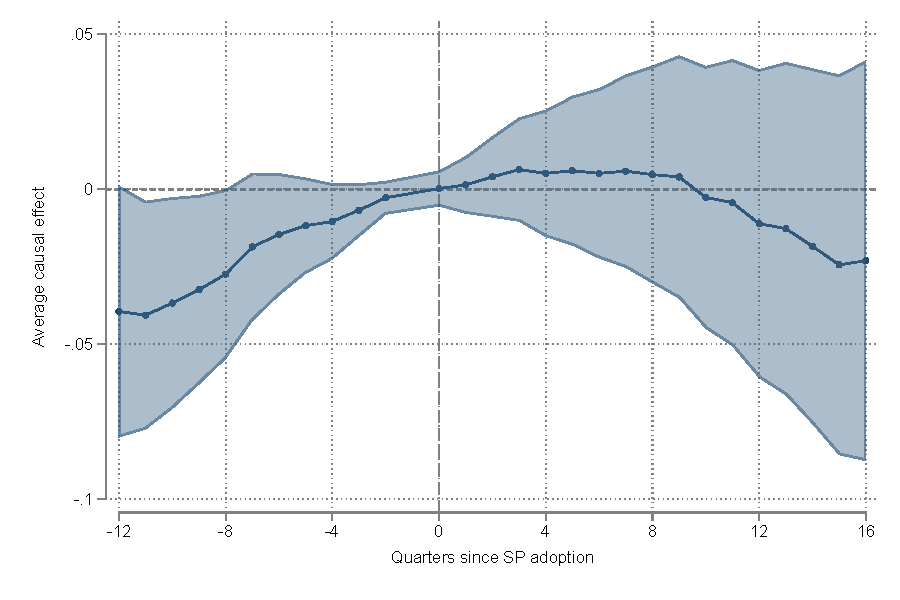
\includegraphics[width=\textwidth]{Figuras/did_event_bc_e_t.pdf}
    \end{subfigure}
  
  \end{center}
    \scriptsize 

%\textit{Scripts: }  \texttt{did\_bc.do}
\end{figure}


\subsection{Robustness analysis of \cite{Campos} specification}


\begin{figure}[H]
     \caption{More municipalities}
    \label{es_more_mun}
\begin{center}
       \begin{subfigure}{0.325\textwidth}
    \caption{Employers}
        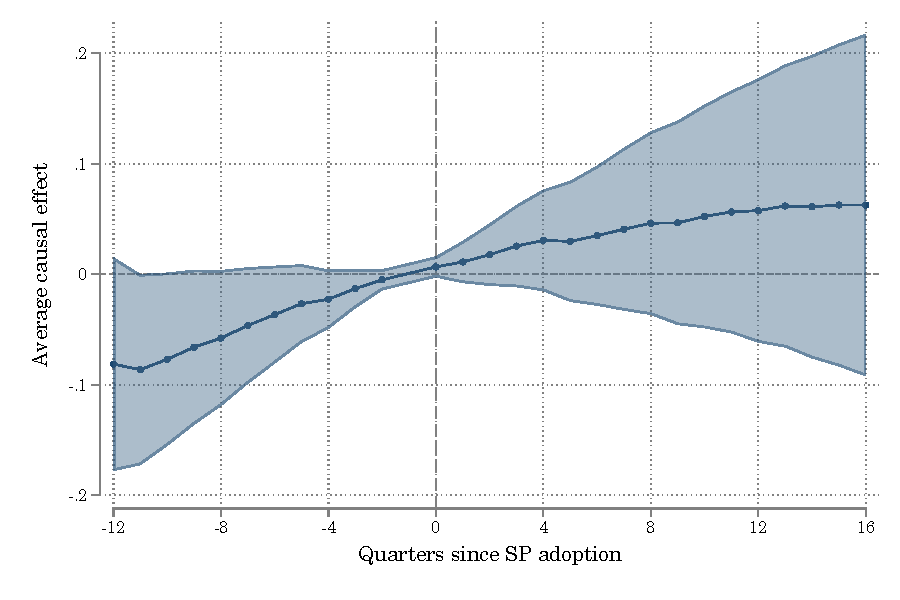
\includegraphics[width=\textwidth]{Figuras/did_event_mun_p_t.pdf}
    \end{subfigure}
    \begin{subfigure}{0.325\textwidth}
        \caption{Self-employed}
        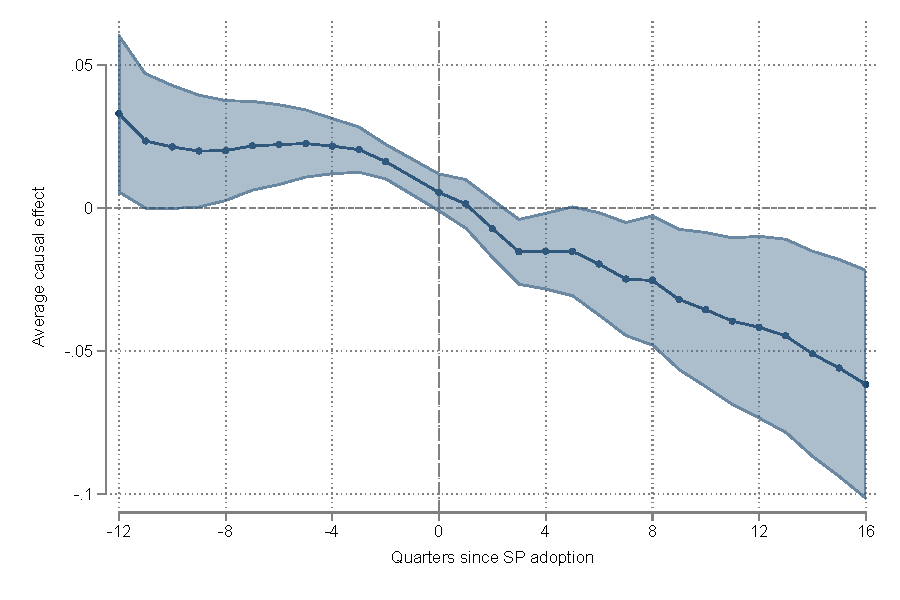
\includegraphics[width=\textwidth]{Figuras/did_event_mun_p_1.pdf}
    \end{subfigure}
        \begin{subfigure}{0.325\textwidth}
    \caption{Employees}
        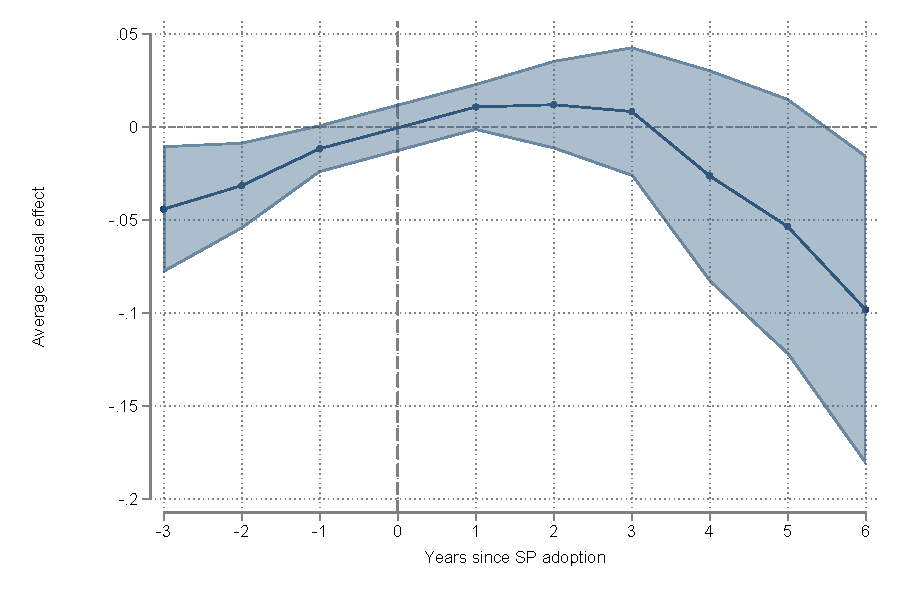
\includegraphics[width=\textwidth]{Figuras/did_event_mun_e_t.pdf}
    \end{subfigure}
  
  \end{center}
    \scriptsize 
%\textit{Scripts: }  \texttt{did\_es.do}
\end{figure}


\begin{figure}[H]
     \caption{Flexible specification}
    \label{es_flex}
\begin{center}
       \begin{subfigure}{0.325\textwidth}
    \caption{Employers}
        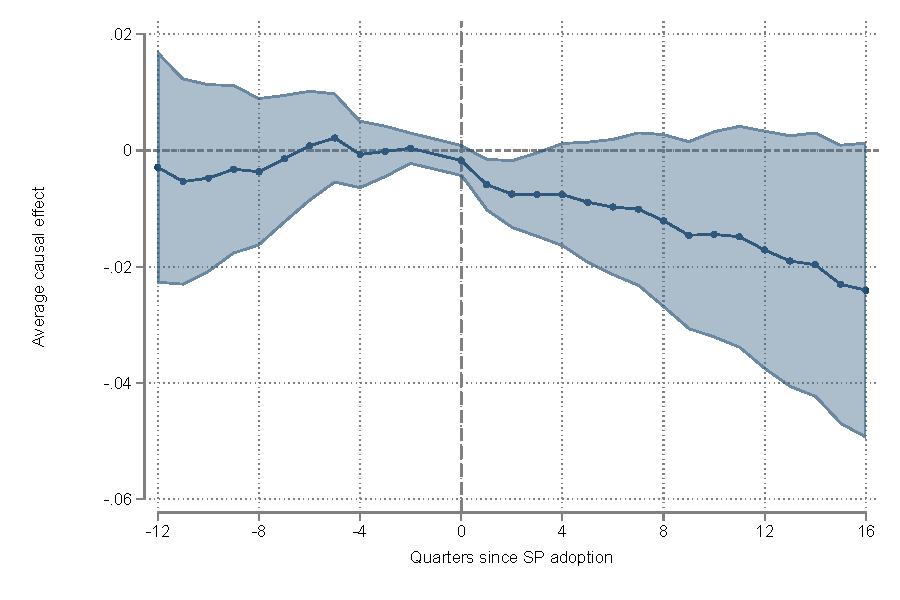
\includegraphics[width=\textwidth]{Figuras/did_event_flex_p_t.pdf}
    \end{subfigure}
    \begin{subfigure}{0.325\textwidth}
        \caption{Self-employed}
        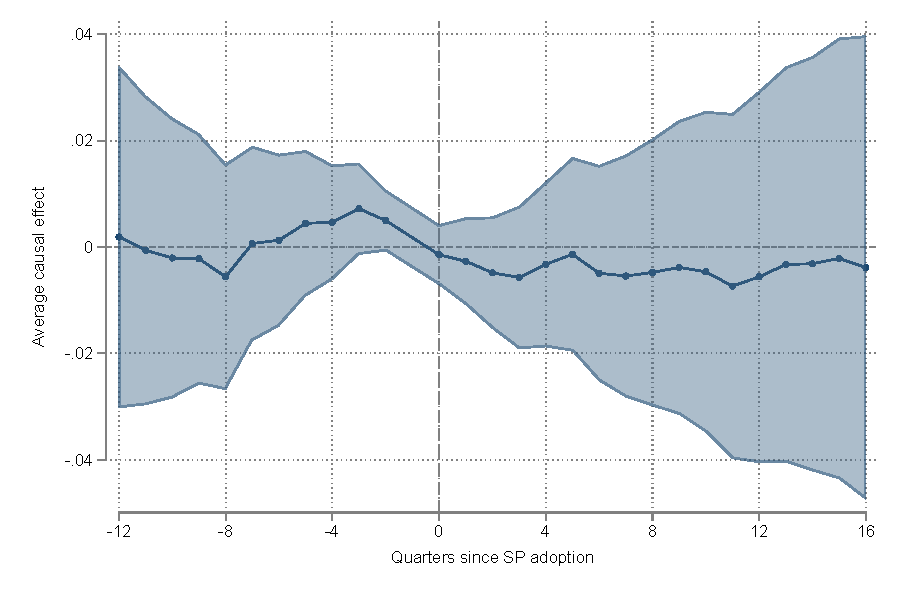
\includegraphics[width=\textwidth]{Figuras/did_event_flex_p_1.pdf}
    \end{subfigure}
        \begin{subfigure}{0.325\textwidth}
    \caption{Employees}
        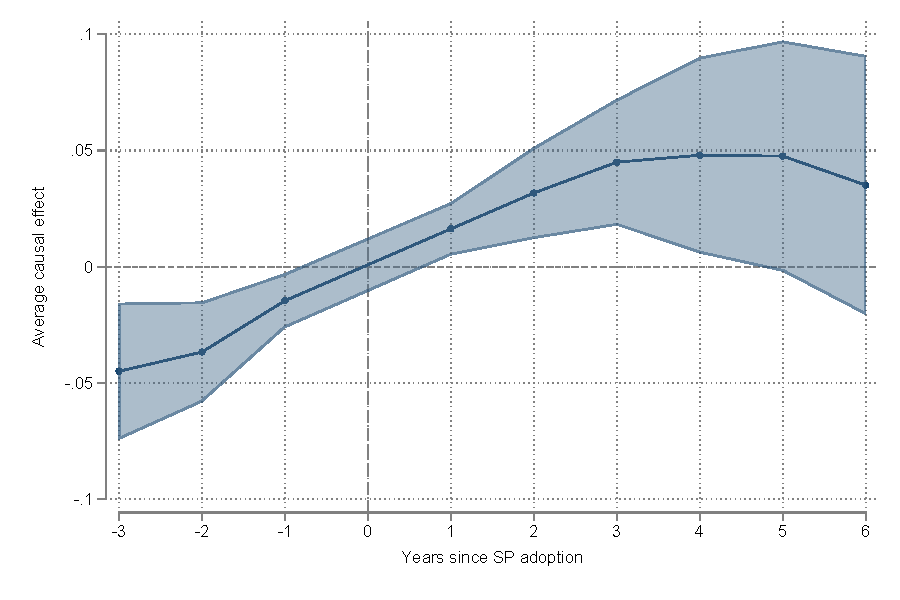
\includegraphics[width=\textwidth]{Figuras/did_event_flex_e_t.pdf}
    \end{subfigure}
  
  \end{center}
    \scriptsize 

%\textit{Scripts: }  \texttt{did\_es.do}
\end{figure}


\newpage

\subsection{Instrumental variables}

\vspace{.2in}
\begin{figure}[H]
     \caption{Clinics in MX}
    \label{map_clinics}
\begin{center}
\begin{subfigure}{0.45\textwidth}
\caption{Clinics in 2004}
        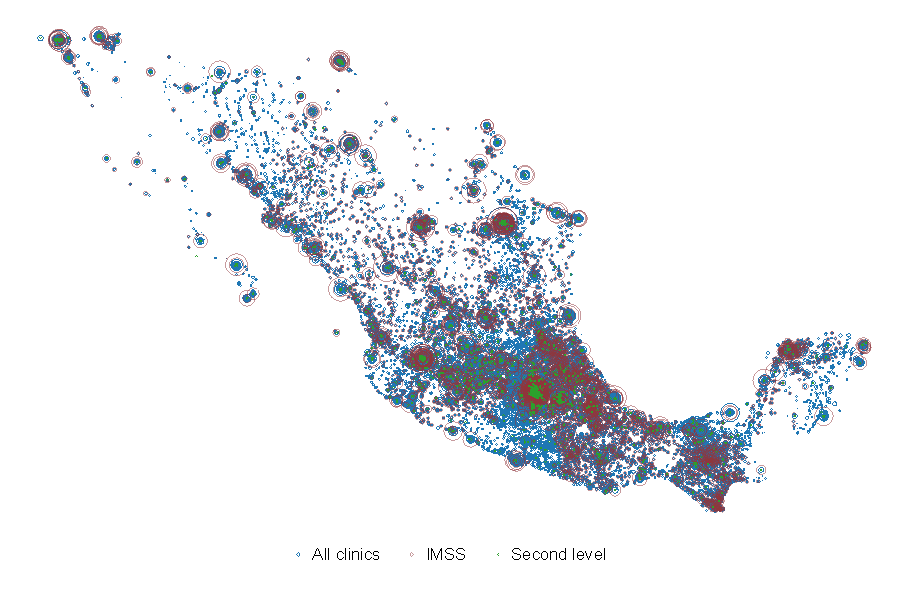
\includegraphics[width=\textwidth]{Figuras/map_clinics_04.pdf}
    \end{subfigure}
\begin{subfigure}{0.45\textwidth}
\caption{New clinics in 2007}
        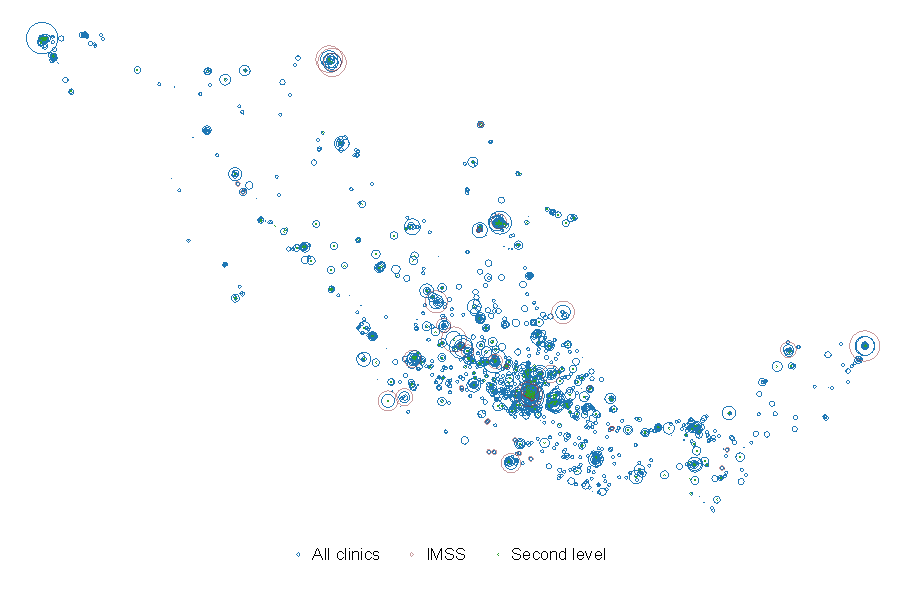
\includegraphics[width=\textwidth]{Figuras/map_clinics_07.pdf}
    \end{subfigure}    
  \end{center}
    \scriptsize 
%\textit{Scripts: }  \texttt{map_clinics.do}
\end{figure}




\vspace{.3in}
\begin{figure}[H]
     \caption{Trends of IMSS employment by terciles of the \# of clinics} \label{trends_clinics}
\begin{center}
    \begin{subfigure}{0.45\textwidth}
    \caption{Total employment}
        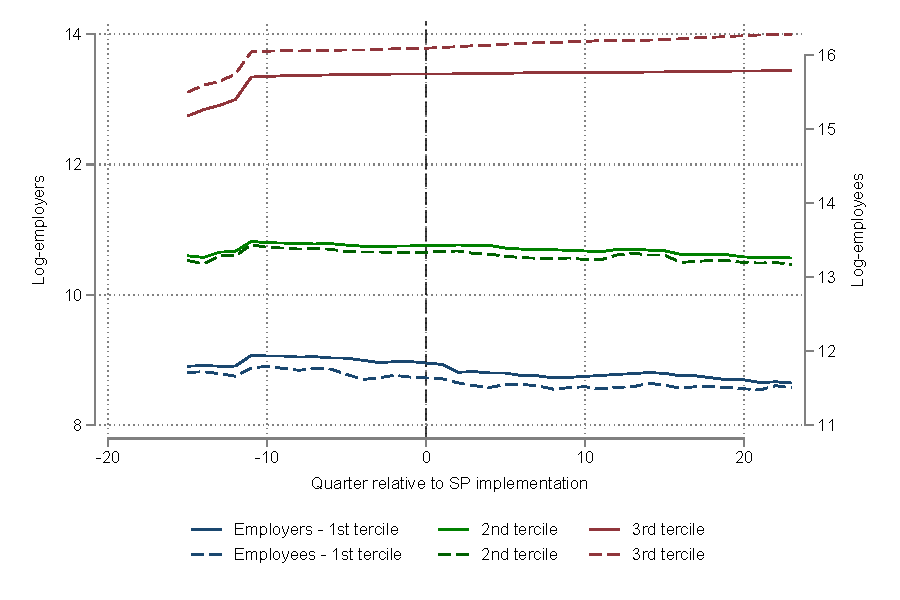
\includegraphics[width=\textwidth]{Figuras/trends_clinics_total.pdf}
    \end{subfigure}
    \begin{subfigure}{0.45\textwidth}
    \caption{Self-employed}
        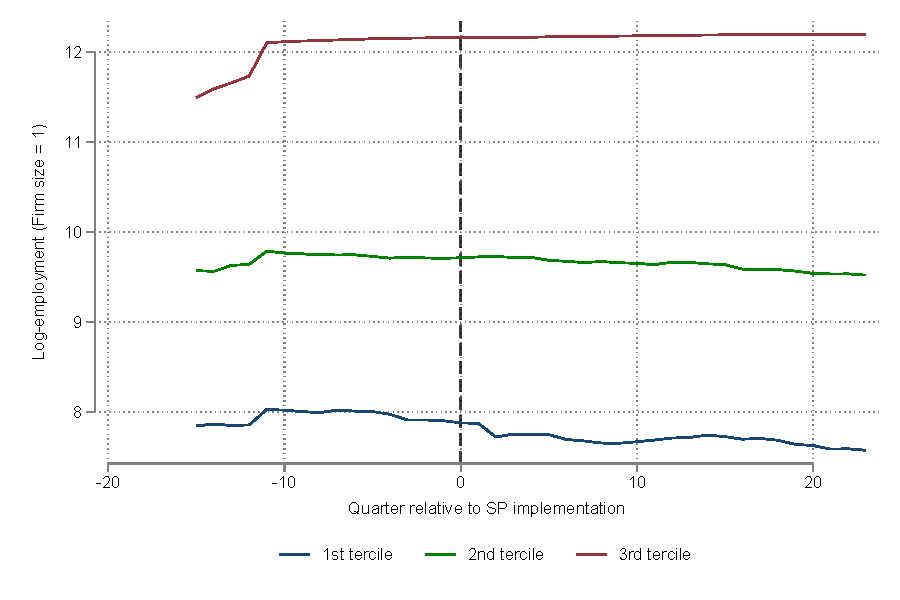
\includegraphics[width=\textwidth]{Figuras/trends_clinics_self.pdf}
    \end{subfigure}
  \end{center}
    
    \scriptsize 
%\textit{Scripts: }  \texttt{trends_emp_clinics.do}
\end{figure}




\begin{table}[H]
\caption{Pre-time trends (1-year)}
\label{pretime_trends}
\begin{center}
\resizebox{0.75\textwidth}{!}{
\scriptsize{% Table generated by Excel2LaTeX from sheet 'pretime_trends_instrument_4q'
\begin{tabular}{lccccccccccc}
\toprule
      & \multicolumn{2}{c}{Employer} &       & \multicolumn{2}{c}{Employee} &       & \multicolumn{2}{c}{Asalaried} &       & \multicolumn{2}{c}{Total wage mass} \\
\cmidrule{2-3}\cmidrule{5-6}\cmidrule{8-9}\cmidrule{11-12}      & (1)   & (2)   &       & (3)   & (4)   &       & (5)   & (6)   &       & (7)   & (8) \\
\midrule
\midrule
Log(Total \# clinics) & -0.019 &       &       & 0.083 &       &       & 0.085 &       &       & 0.037 &  \\
      & (0.033) &       &       & (0.071) &       &       & (0.071) &       &       & (0.057) &  \\
Log(\# IMSS clinics) & 0.015 &       &       & -0.016 &       &       & -0.032 &       &       & 0.058 &  \\
      & (0.016) &       &       & (0.032) &       &       & (0.033) &       &       & (0.046) &  \\
Log(\# 2nd level clinic) & -0.0030 &       &       & -0.016 &       &       & -0.018 &       &       & -0.033 &  \\
      & (0.018) &       &       & (0.032) &       &       & (0.032) &       &       & (0.035) &  \\
Log(\# 3rd level clinic) & 0.014 &       &       & -0.066** &       &       & -0.066** &       &       & -0.11** &  \\
      & (0.015) &       &       & (0.031) &       &       & (0.030) &       &       & (0.044) &  \\
Log(Total \# of rooms) & -0.070 &       &       & -0.11 &       &       & -0.095 &       &       & 0.0083 &  \\
      & (0.044) &       &       & (0.095) &       &       & (0.095) &       &       & (0.055) &  \\
Log(Total \# of beds) & -0.00081 &       &       & 0.028* &       &       & 0.018 &       &       & 0.025* &  \\
      & (0.0070) &       &       & (0.015) &       &       & (0.014) &       &       & (0.015) &  \\
PAN   & -0.0074 &       &       & -0.017 &       &       & -0.0049 &       &       & -0.0038 &  \\
      & (0.0067) &       &       & (0.015) &       &       & (0.015) &       &       & (0.020) &  \\
PRD   & 0     &       &       & 0     &       &       & 0     &       &       & 0     &  \\
      & (.)   &       &       & (.)   &       &       & (.)   &       &       & (.)   &  \\
\midrule
Log-population & -0.0081 & -0.061 &       & -0.33*** & -0.18** &       & -0.36*** & -0.17* &       & -0.69*** & -0.62*** \\
      & (0.050) & (0.038) &       & (0.12) & (0.085) &       & (0.13) & (0.092) &       & (0.15) & (0.098) \\
$\text{Luminosity}$ & 0.0041 & -0.0053 &       & 0.014** & 0.0028 &       & 0.017** & 0.0023 &       & 0.0063 & -0.026*** \\
      & (0.0034) & (0.0034) &       & (0.0073) & (0.0070) &       & (0.0081) & (0.0079) &       & (0.0088) & (0.0086) \\
$\text{Luminosity}^2$ & 0.000072 & 0.00012 &       & -0.00072** & -0.00062** &       & -0.00063** & -0.00058* &       & -0.000042 & 0.000080 \\
      & (0.00014) & (0.00014) &       & (0.00028) & (0.00028) &       & (0.00030) & (0.00030) &       & (0.00029) & (0.00029) \\
$\text{Luminosity}^3$ & -0.0000014 & -0.00000056 &       & 0.0000098*** & 0.000010*** &       & 0.0000084** & 0.0000096*** &       & 0.0000021 & 0.0000058* \\
      & (0.0000016) & (0.0000016) &       & (0.0000034) & (0.0000034) &       & (0.0000036) & (0.0000035) &       & (0.0000032) & (0.0000032) \\
Gender & -0.30*** & -0.37*** &       & -0.92*** & -1.01*** &       & -0.97*** & -1.10*** &       & -0.82*** & -1.07*** \\
      & (0.044) & (0.042) &       & (0.12) & (0.12) &       & (0.12) & (0.12) &       & (0.12) & (0.12) \\
Wage  & 0.00033*** & -0.00036*** &       & 0.0029*** & 0.0021*** &       & 0.0030*** & 0.0021*** &       & 0.0067*** & 0.0044*** \\
      & (0.00011) & (0.000088) &       & (0.00040) & (0.00027) &       & (0.00041) & (0.00028) &       & (0.00043) & (0.00028) \\
      &       &       &       &       &       &       &       &       &       &       &  \\
\midrule
Observations & 23200 & 23200 &       & 23200 & 23200 &       & 23402 & 23402 &       & 23464 & 23464 \\
R-sq  & 0.163 & 0.151 &       & 0.173 & 0.164 &       & 0.233 & 0.224 &       & 0.471 & 0.457 \\
F-statistics & 22.5  & 19.7  &       & 8.53  & 21.8  &       & 9.17  & 24.0  &       & 11.9  & 53.5 \\
p-value & 0.0013 &       &       & 0.090 &       &       & 0.081 &       &       & 0.15  &  \\
Municipality FE & \checkmark & \checkmark &       & \checkmark & \checkmark &       & \checkmark & \checkmark &       & \checkmark & \checkmark \\
LASSO selection &       & \checkmark &       &       & \checkmark &       &       & \checkmark &       &       & \checkmark \\
\bottomrule
\bottomrule
\end{tabular}%
}
}
\end{center}
 \scriptsize 
 In this table we test for the exclusion restriction of our instrument(s). This assumption states that the instruments are uncorrelated with outcome (employment) except that through its effect of SP implementation. To `test' for this assumption we estimate 
 $\log{\frac{y_{t+1}}{y_t}} = \alpha + \beta_kZ_{k,t} + \epsilon_{t}$ 
 in the pre-implementation periods.  Our hypothesis is that $\beta_k=0$. Odd-numbered columns estimates the previous equation and does not reject $H_0 : \beta_k = 0$. Even-numbered columns runs same specification but with variable selection using Lasso.
 
%\textit{Do file: } \texttt{iv\_sp.do}
\end{table}



\begin{figure}[H]
     \caption{First stage}
     \vspace{-.2in}
    \label{iv_fs}
\begin{center}
\begin{subfigure}{0.4\textwidth}
        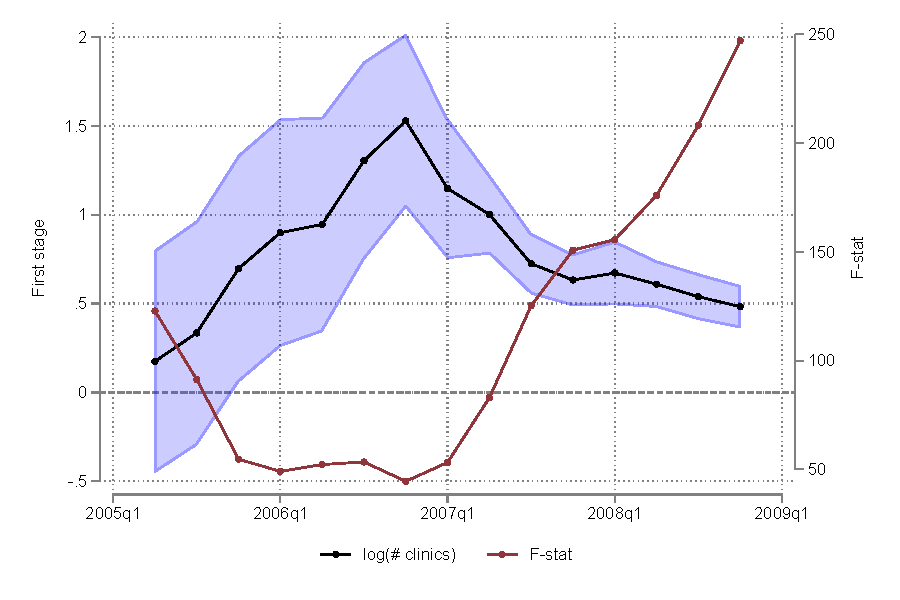
\includegraphics[width=\textwidth]{Figuras/IV_FS.pdf}
    \end{subfigure}
  \end{center}
  \vspace{-.15in}
    \scriptsize 
   This figure shows the F-statistic and an estimated coefficient for the first stage plotted for each quarter. Error are clustered at municipality level.
    
%\textit{Scripts: }  \texttt{iv_sp.do}
\end{figure}



\begin{figure}[H]
     \caption{Dynamic second stage}
     \vspace{-.2in}
    \label{iv_sp_dynamic}
\begin{center}
\begin{subfigure}{0.325\textwidth}
\caption{Employer}
        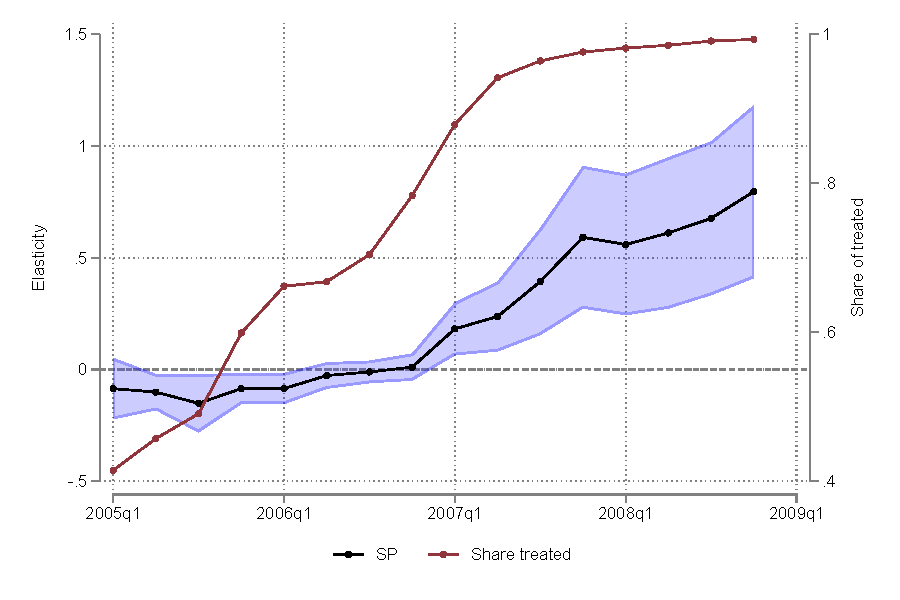
\includegraphics[width=\textwidth]{Figuras/IV_SP_p_t_.pdf}
    \end{subfigure}
\begin{subfigure}{0.325\textwidth}
\caption{Self-employed}
        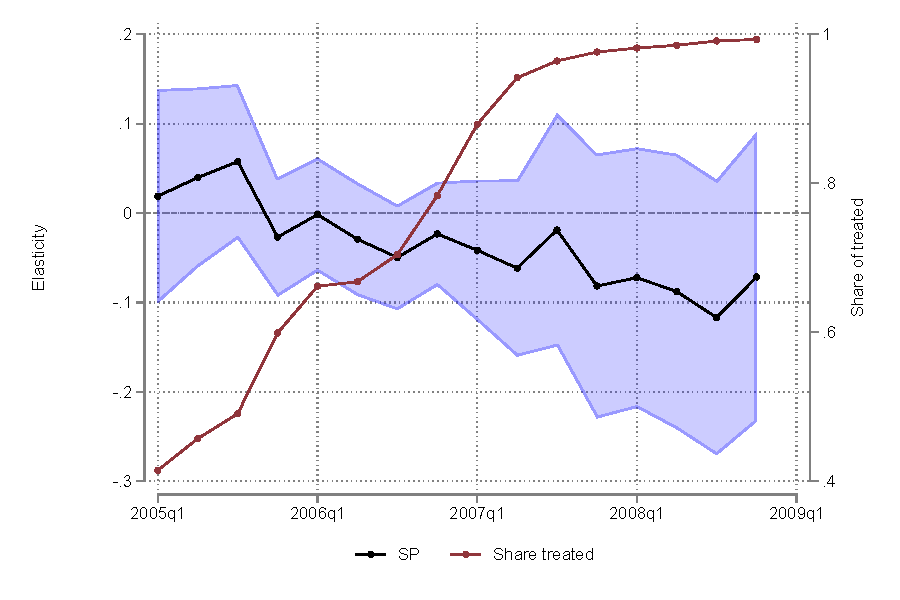
\includegraphics[width=\textwidth]{Figuras/IV_SP_p_1_.pdf}
    \end{subfigure}
\begin{subfigure}{0.325\textwidth}
\caption{Employee}
        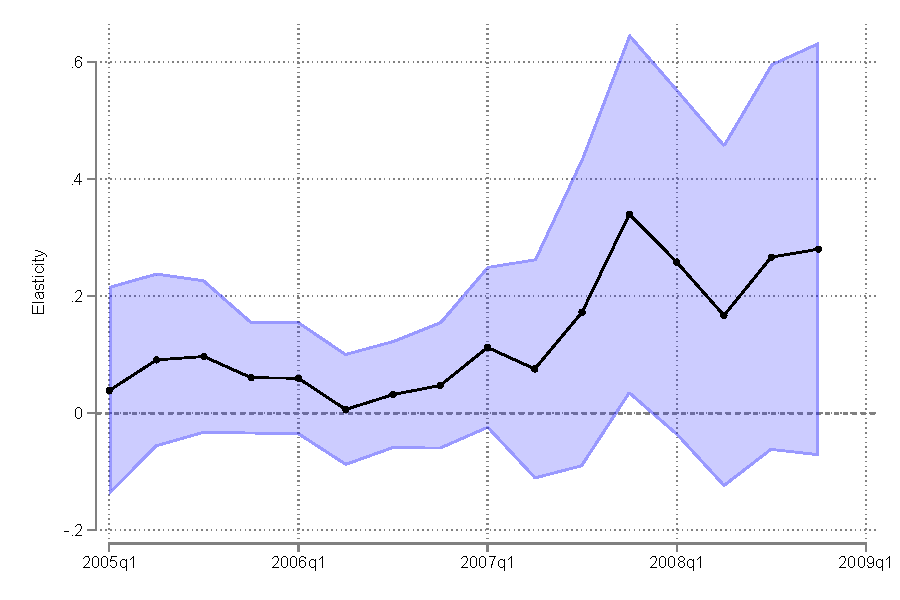
\includegraphics[width=\textwidth]{Figuras/IV_SP_e_t_.pdf}
    \end{subfigure}  
  \end{center}
  \vspace{-.15in}
    \scriptsize 
   This figure shows second stage separately for each quarter using the first stage from Figure \ref{iv_fs}. Error are clustered at municipality level.
    
%\textit{Scripts: }  \texttt{iv_sp.do}
\end{figure}

\vspace{2in}



\subsection{Difference of salaries for IMSS/no IMSS}

\begin{table}[H]
\caption{Salary changes}
\label{salary_changes}
\begin{center}
\resizebox{0.40\textwidth}{!}{
\scriptsize{% Table generated by Excel2LaTeX from sheet 'consequences_informal'
\begin{tabular}{lccccc}
\toprule
      & \multicolumn{2}{c}{[2005, 2010]} &       & \multicolumn{2}{c}{[2010, 2015]} \\
\cmidrule{2-3}\cmidrule{5-6}      & Log(hourly wage) & Weekly hours &       & Log(hourly wage) & Weekly hours \\
\midrule
      & (1)   & (2)   &       & (3)   & (4) \\
\midrule
\midrule
No IMSS & -0.23*** & -5.79*** &       & -0.15*** & -6.50*** \\
      & (0.00) & (0.00) &       & (0.00) & (0.00) \\
Woman & -0.12*** & -7.33*** &       & -0.06*** & -7.21*** \\
      & (0.00) & (0.00) &       & (0.00) & (0.00) \\
Age   & -0.00*** & 0.01*** &       & -0.00*** & 0.00*** \\
      & (0.00) & (0.00) &       & (0.00) & (0.00) \\
Years of schooling & 0.01*** & 0.04*** &       & -0.01*** & 0.03*** \\
      & (0.00) & (0.00) &       & (0.00) & (0.00) \\
Married & 0.25*** & 1.59*** &       & 0.23*** & 1.50*** \\
      & (0.00) & (0.00) &       & (0.00) & (0.00) \\
      &       &       &       &       &  \\
\midrule
Obs   & 3.376e+06 & 3.376e+06 &       & 3.991e+06 & 3.991e+06 \\
Population & 887,534,856 & 887,534,856 &       & 1169577977 & 1169577977 \\
R-squared & 0.18  & 0.16  &       & 0.14  & 0.17 \\
Dep var mean & 2.272 & 41.29 &       & 2.213 & 41.21 \\
Municipality $\times$ Date FE & \checkmark & \checkmark &       & \checkmark & \checkmark \\
Occupation FE & \checkmark & \checkmark &       & \checkmark & \checkmark \\
\bottomrule
\bottomrule
\end{tabular}%
}
}
\end{center}
\scriptsize 
% \textit{Do file: } \texttt{consequences\_informal.do}
\end{table}


\newpage 


